\documentclass[8pt,a4paper]{beamer}

% PACKAGES
\usepackage[utf8]{inputenc}
\usepackage[T1]{fontenc}
\usepackage[francais]{babel}
%\usepackage{ucs} % Utilisation de l'unicode
%\usepackage{amsmath}
%\usepackage{amsfonts}
%\usepackage{amssymb}
\usepackage{graphicx}
\usepackage{fancybox}
%\usepackage{multimedia}
\usepackage{ragged2e} % Pour les textes justifiés
\usepackage{listings} % Intégration de listings de programmes
\usepackage{hyperref}

% CONFIGURATION DES PACKAGES
\hypersetup{
    bookmarks=true,         % show bookmarks bar?
    pdftoolbar=true,        % show Acrobat’s toolbar?
    pdfmenubar=true,        % show Acrobat’s menu?
    colorlinks=false,       % false: boxed links; true: colored links
    linkcolor=red,          % color of internal links
    citecolor=green,        % color of links to bibliography
    filecolor=magenta,      % color of file links
    urlcolor=cyan           % color of external links
}

% ragged2e
\justifying

% Listings
\lstset{ %
language=Python,                % the language of the code
basicstyle=\footnotesize,       % the size of the fonts that are used for the code
numbers=left,                   % where to put the line-numbers
numberstyle=\footnotesize,      % the size of the fonts that are used for the line-numbers
stepnumber=1,                   % the step between two line-numbers. If it's 1, each line 
                                % will be numbered
numbersep=5pt,                  % how far the line-numbers are from the code
backgroundcolor=\color{white},  % choose the background color. You must add \usepackage{color}
showspaces=false,               % show spaces adding particular underscores
showstringspaces=false,         % underline spaces within strings
showtabs=false,                 % show tabs within strings adding particular underscores
frame=single,                   % adds a frame around the code
tabsize=2,                      % sets default tabsize to 2 spaces
captionpos=b,                   % sets the caption-position to bottom
breaklines=true,                % sets automatic line breaking
breakatwhitespace=false,        % sets if automatic breaks should only happen at whitespace
keywordstyle=\color{red}\bfseries,  	% underlined bold black keywords
identifierstyle=,						% nothing happens
commentstyle=\color{gray}, 				% white comments
stringstyle=\ttfamily					% typewriter type for strings
}

% THEME

\usetheme{Frankfurt}
%\usetheme{Montpellier}
%\usetheme{Hannover}
%\usecolortheme{wolverine}
%\usetheme{Antibes}
%\usecolortheme{beaver}
%\usecolortheme{seahorse}
%\usecolortheme{dolphin}
%\useoutertheme{infolines}

% MODIFICATIONS DIVERSES
\setcounter{tocdepth}{1}
\setbeamertemplate{footline}[page number]
 %Gestion du numero de page
\setbeamertemplate{footline}
{%
\leavevmode%
\hbox{%
\begin{beamercolorbox}[wd=.5\paperwidth,ht=2.5ex,dp=1.125ex,right]{author
in head/foot}%
%\usebeamerfont{title in head/foot}\inserttitle\hspace{.3cm}
\usebeamerfont{title in head/foot}Outils numériques pour l'ingénieur\hspace{.3cm}
\end{beamercolorbox}%
\begin{beamercolorbox}[wd=.4\paperwidth,ht=2.5ex,dp=1.125ex,left]{title
in head/foot}%
\usebeamerfont{author in head/foot}\hspace{.3cm}\insertdate
\end{beamercolorbox}%
\begin{beamercolorbox}[wd=.1\paperwidth,ht=2.5ex,dp=1.125ex,center]{title
in head/foot}%
\usebeamerfont{author in
head/foot}\insertframenumber/\inserttotalframenumber
\end{beamercolorbox}%
}%
\vskip0pt%
}


%\renewcommand\Re{\operatorname{Re}}
%\renewcommand\Im{\operatorname{Im}}

\AtBeginSection[]
{
\begin{frame}{Plan}
\tableofcontents[currentsection]
\end{frame}
}



\author[LC]{\href{mailto:ludovic.charleux@univ-savoie.fr}{ludovic.charleux@univ-savoie.fr}}
\title{MGM657 Outils Numériques pour l'Ingénieur}
\subtitle{Traitement d'Images}
%\subtitle{}
\date{}
\institute{\url{www.polytech.univ-savoie.fr}}


% DEBUT DU DOCUMENT
\begin{document}

% PAGE DE GARDE
\begin{frame}[plain]
%\begin{columns}[c]
%\column{.5\textwidth}
%\center{\includegraphics[width=.75\textwidth]{figures/logo_polytech.jpg}}
%\column{.5\textwidth}
%\center{\includegraphics[width=.75\textwidth]{figures/logo_univ-savoie.jpg}}
%\end{columns}
\titlepage
\tableofcontents
\end{frame}

\section{Ouverture/Fermeture}
  
\begin{frame}[containsverbatim]{Lire et afficher une image}
  \begin{columns}
  \column{.47\textwidth}
  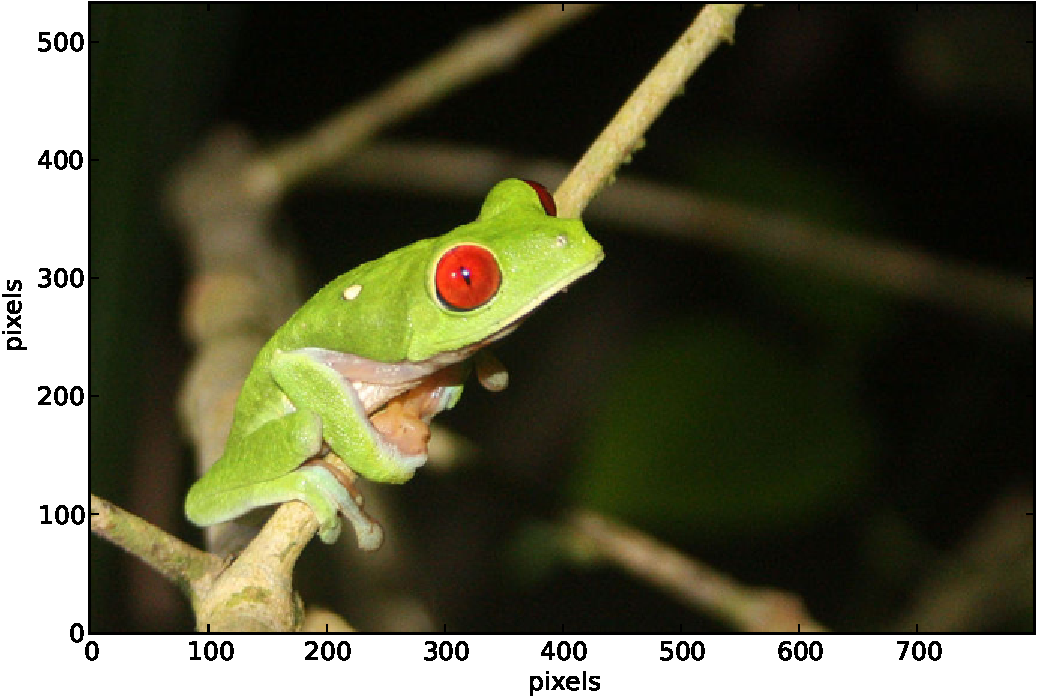
\includegraphics[width=\textwidth]{figures/grenouille.pdf} 
  \column{.47\textwidth} 
  \lstinputlisting{../Example_code/grenouille.py}
  \end{columns}
  \begin{block}{Points clés}
  \begin{itemize}
  \item \verb!PIL! : utile pour lire et écrire divers formats d'images.
  \item \verb!Matplotlib!: permet d'afficher les images
  \end{itemize}
  \end{block}
\end{frame}


\begin{frame}[containsverbatim]{Canaux et couleurs}
  \begin{columns}
  \column{.32\textwidth}
  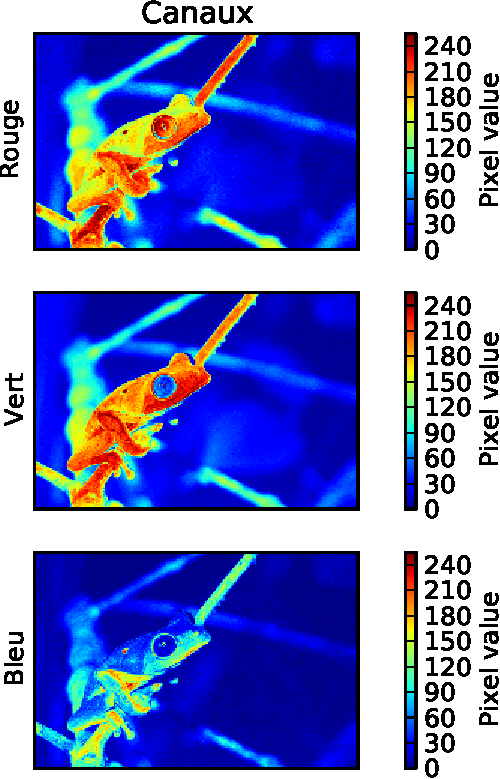
\includegraphics[width=\textwidth]{figures/grenouille_canaux.pdf} 
  \column{.62\textwidth} 
  \lstinputlisting[lastline=8]{../Example_code/grenouille_canaux.py}
  \begin{block}{Types d'images}
  \begin{itemize}
  \item Canal: 1 information (entier 8 bits)
  \item Image couleur: 3(+1) canaux 
  \item Imagerie monochrome: 1 canal
  \end{itemize}
  \end{block}  
  \end{columns}
  \begin{alertblock}{Remarque}
  \begin{itemize}
  \item Contexte scientifique: généralement un seul canal.
  \item On peut afficher une image monochrome avec une échelle de couleurs.
  \end{itemize}
  
  \end{alertblock}
  
\end{frame}

\begin{frame}[containsverbatim]{Image = \verb!np.array!}
  \lstinputlisting{../Example_code/grenouille_array.py}  
  \begin{lstlisting}[language=Python]
>>> z
array([[16, 17, 19, ..., 10,  9,  8],
       [14, 15, 17, ..., 10,  9,  8],
       [15, 16, 18, ..., 11,  9,  8],
       ..., 
       [25, 24, 24, ..., 19, 20, 20],
       [24, 23, 23, ..., 17, 19, 19],
       [23, 23, 22, ..., 18, 18, 18]], dtype=uint8)
>>> z.shape
(534, 800)
>>> nx, ny = z.shape
>>> z.dtype
dtype('uint8')
\end{lstlisting}
\end{frame}


\begin{frame}[containsverbatim]{Sauvegarde}
  \begin{center}
  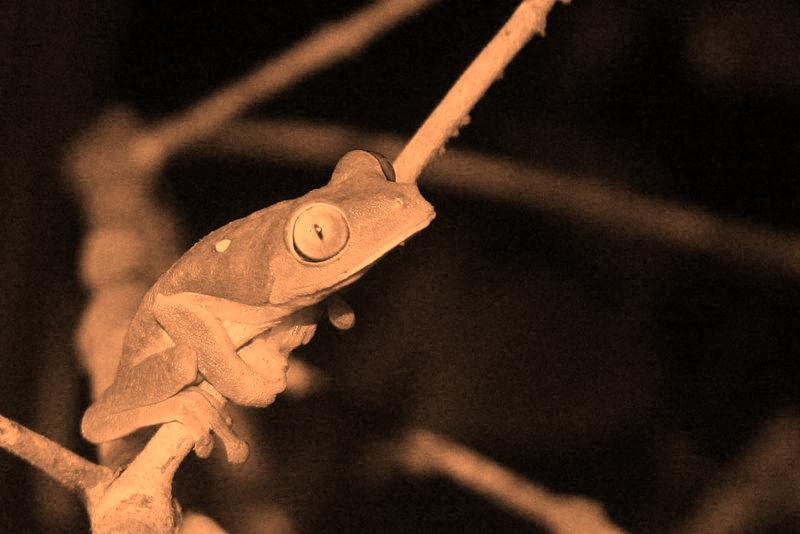
\includegraphics[width=.6\textwidth]{figures/grenouille_saved.jpg} 
  \end{center}    
  \lstinputlisting{../Example_code/grenouille_save.py}
\end{frame}



\section{Opérations basiques}

\begin{frame}[containsverbatim]{Rognage (\textit{Crop})}
  \begin{columns}
  \column{.42\textwidth}
  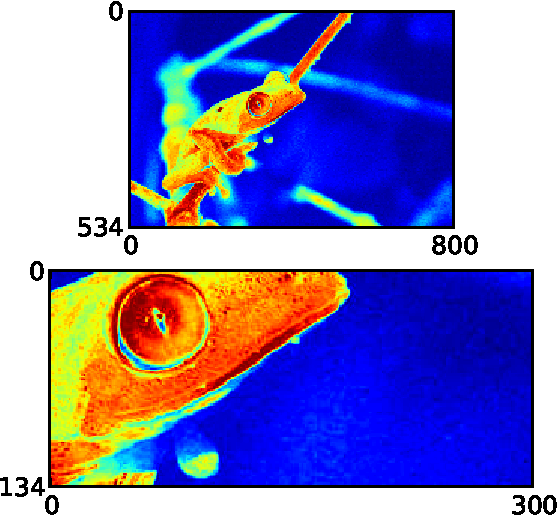
\includegraphics[width=\textwidth]{figures/grenouille_crop.pdf} 
  \column{.58\textwidth} 
  \lstinputlisting[lastline=23]{../Example_code/grenouille_crop.py}
    \end{columns}
\end{frame}


\begin{frame}[containsverbatim]{Rotation}
  \begin{columns}
  \column{.35\textwidth}
  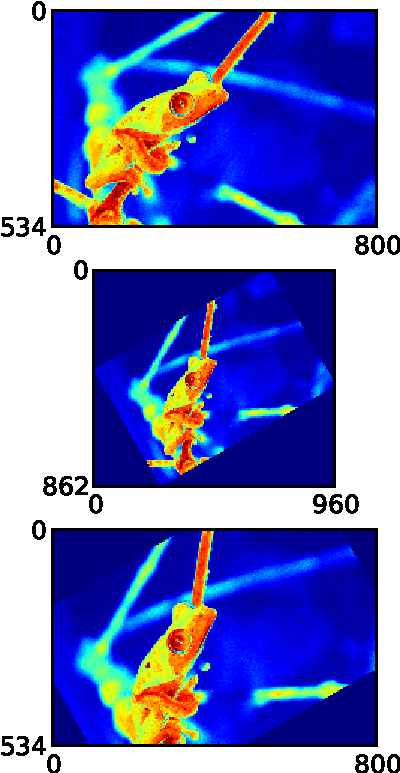
\includegraphics[width=\textwidth]{figures/grenouille_rotate.pdf} 
  \column{.65\textwidth} 
  \lstinputlisting[lastline=23]{../Example_code/grenouille_rotate.py}
    \end{columns}
\end{frame}  


\section{Filtrage}

\begin{frame}[containsverbatim]{Lissage: exemple sur un signal 1D}
  \begin{center}
  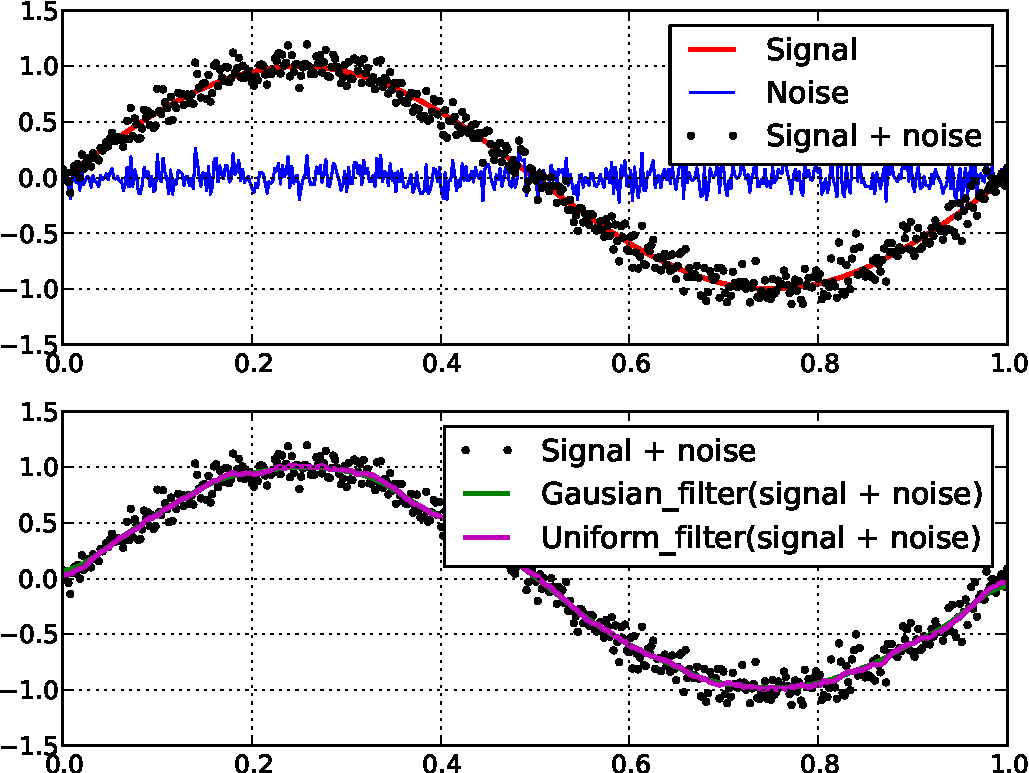
\includegraphics[width=.6\textwidth]{figures/filters.pdf} 
  \end{center}  
  \lstinputlisting[lastline=9]{../Example_code/filters.py}
\end{frame}  

\begin{frame}[containsverbatim]{Lissage image}
  \begin{columns}
  \column{.35\textwidth}
  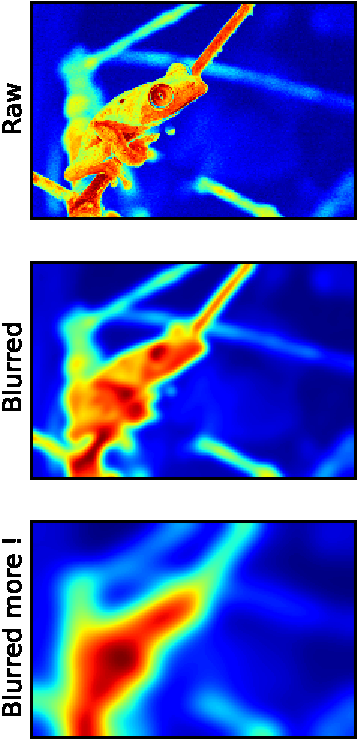
\includegraphics[width=\textwidth]{figures/grenouille_lissage.pdf} 
  \column{.65\textwidth} 
  \lstinputlisting[lastline=11]{../Example_code/grenouille_lissage.py}
    \end{columns}
\end{frame}  


\begin{frame}[containsverbatim]{Histogramme}
  \begin{columns}
  \column{.35\textwidth}
  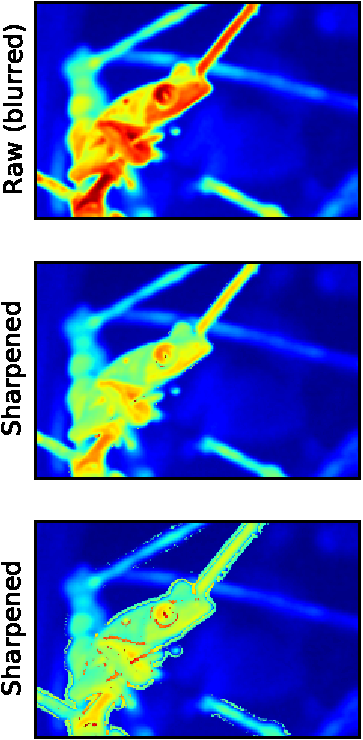
\includegraphics[width=\textwidth]{figures/grenouille_sharpen.pdf} 
  \column{.65\textwidth} 
  \lstinputlisting[lastline=11]{../Example_code/grenouille_sharpen.py}
    \end{columns}
\end{frame}  

\section{Histogramme}

\begin{frame}[containsverbatim]{Histogramme}
  \begin{columns}
  \column{.5\textwidth}
  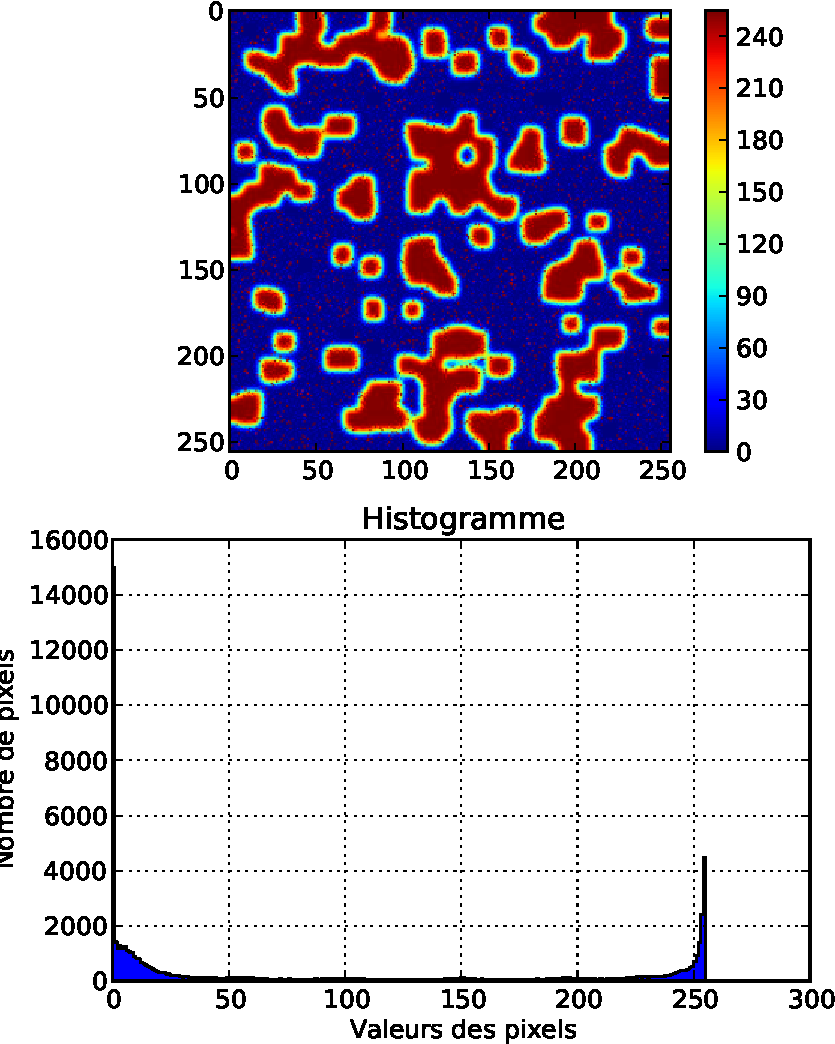
\includegraphics[width=\textwidth]{figures/histogram.pdf} 
  \column{.5\textwidth} 
  \lstinputlisting{../Example_code/image_hist.py}
    \end{columns}
\end{frame}  


\section{Seuillage}

\begin{frame}[containsverbatim]{Seuillage}
  \begin{columns}
  \column{.45\textwidth}
  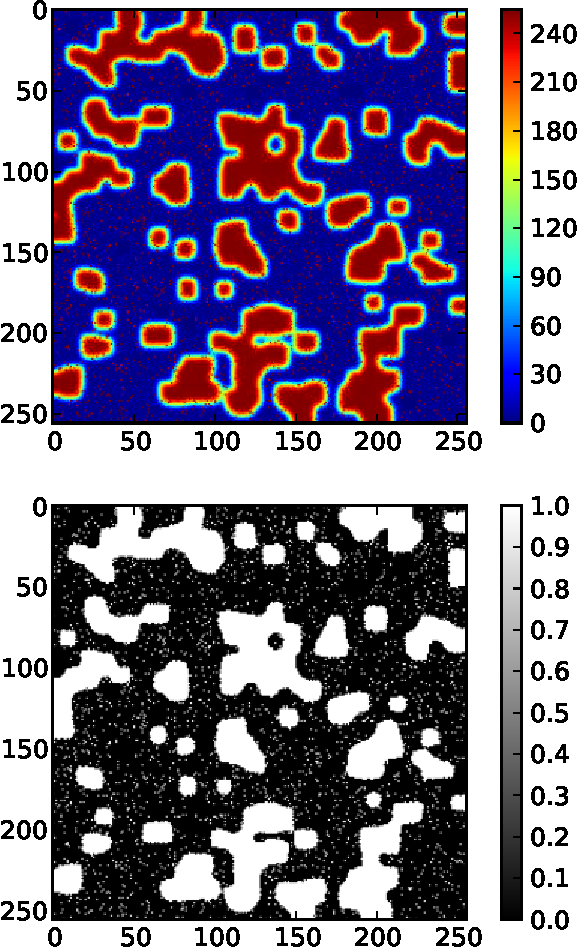
\includegraphics[width=\textwidth]{figures/seuillage.pdf} 
  \column{.55\textwidth} 
  \lstinputlisting{../Example_code/image_seuillage.py}
    \end{columns}
\end{frame}  

\section{Érosion / Dilatation}

\begin{frame}[containsverbatim]{Érosion}
  \begin{columns}
  \column{.45\textwidth}
  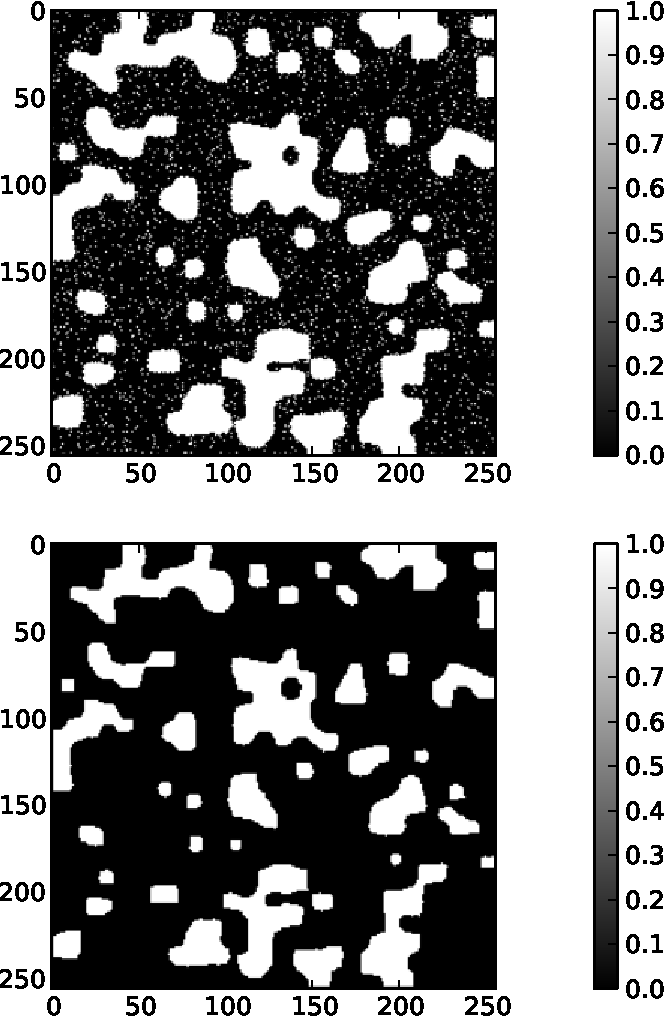
\includegraphics[width=\textwidth]{figures/erosion.pdf} 
  \column{.55\textwidth} 
  \lstinputlisting{../Example_code/image_erosion.py}
    \end{columns}
\end{frame}  

\begin{frame}[containsverbatim]{Dilatation}
  \begin{columns}
  \column{.45\textwidth}
  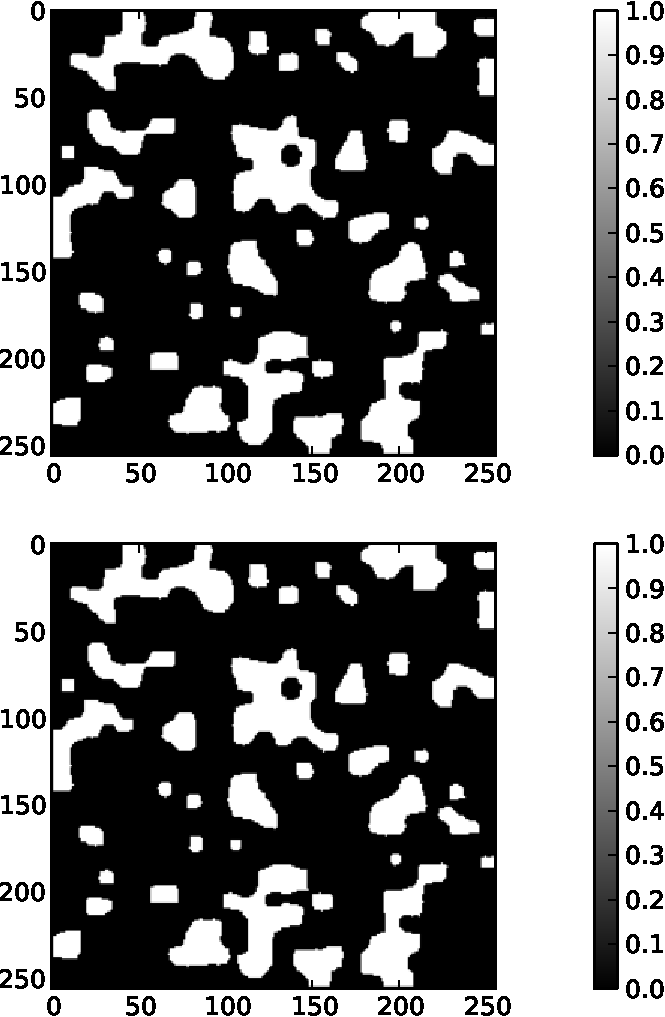
\includegraphics[width=\textwidth]{figures/dilatation.pdf} 
  \column{.55\textwidth} 
  \lstinputlisting{../Example_code/image_dilatation.py}
    \end{columns}
\end{frame}  

\section{Comptage}

\begin{frame}[containsverbatim]{Comptage}
  \begin{columns}
  \column{.45\textwidth}
  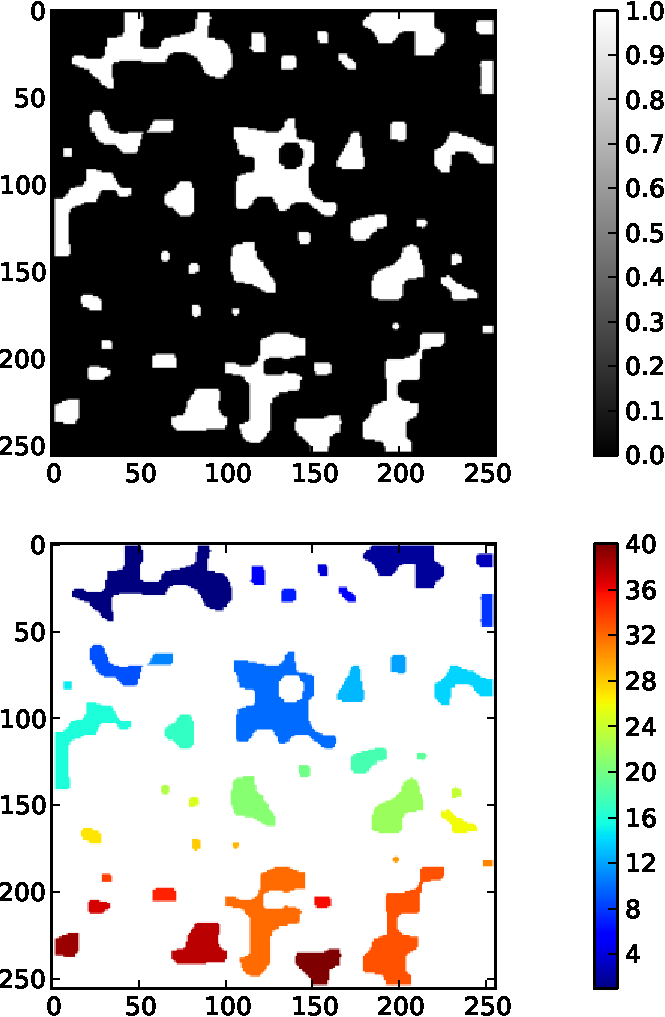
\includegraphics[width=\textwidth]{figures/comptage.pdf} 
  \column{.55\textwidth} 
  \lstinputlisting{../Example_code/image_comptage.py}
    \end{columns}
\end{frame}  

\section{Contours}

\begin{frame}[containsverbatim]{Contours}
  \begin{columns}
  \column{.4\textwidth}
  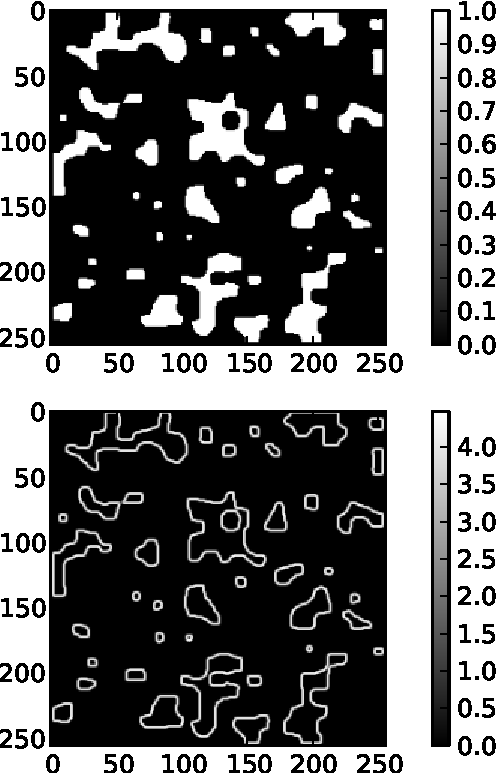
\includegraphics[width=\textwidth]{figures/contours.pdf} 
  \column{.6\textwidth} 
  \lstinputlisting[lastline=15]{../Example_code/image_contours.py}
    \end{columns}
\end{frame}  

\end{document}




